\vspace*{4cm}
\begin{center}
\part{Point to Point Testinfrastruktur}\label{PointtoPointTestinfrastruktur}
\end{center}
\vspace*{\fill}
\clearpage

\section{P2P Messung}\label{sec:P2PMessung}

Im Nachfolgenden Abschnitt wird auf die Point to Point (P2P) Messung eingegangen. Ziel ist es die Verbindung auf MAC-Layer auszumessen. Eine Mac-Layer Verbindung beschreibt die rudimentäre Kommunikation direkt über der physikalischen-Schicht. Dazu wird im folgenden auf das Messkonzept, den Messablauf und technische Einzelheiten eingegangen. 

\subsection{MAC-Layer}\label{sec:MAC-LayerP2P}

Der MAC-Layer ist bei drahtlosen Protokollen oftmals über Normen spezifiziert. Die Hardware-Platfrom (siehe Abschnitt \ref{sec:HardwarePlattform}) unterstützt BLE, sowie den IEEE802.15.4 Standard. Dieser Modus wird im weiteren als Radio-Mode bezeichnet. Nebst dem Mode charakterisiert sich die MAC-Schicht über den verwendeten Kanal. Dabei handelt es sich um eine Frequenz über welche gesendet wird. 

\subsection{Anforderungen}\label{sec:AnforderungentP2P}

Die Anforderungen an die Testinfrastruktur ist es eine Verbindung mit den folgenden Messdaten charakterisieren zu können. 

\begin{itemize}
	\item \textit{\textbf{SNR}} (Signal to Noise Ratio)
	\item \textit{\textbf{Packetloss}} (Paketverlust)
\end{itemize}

Das Ausmessen der obigen Eingenschaften soll pro Kanal (Frequenz) möglich sein. Die folgenden Parameter können vom Benutzer eingestellt werden um eine Messung durchzuführen.

\begin{itemize}
	\item \textit{\textbf{Radio-Mode}} (BLE-1Mbit, IEEE802.15.4, etc.)
	\item \textit{\textbf{Start-Channel}} Abhängig vom Radio-Mode. Kanal ab welchem mit Messen begonnen wird.
	\item \textit{\textbf{Stop-Channel}} Abhängig vom Radio-Mode. Kanal bis zu welchem gemessen wird. 
	\item \textit{\textbf{Tx-Power}} Sendeleistung, mit welcher gesendet wird. 
	\item \textit{\textbf{CA}} Collision-Avoidance-Modus (nur bei IEEE802.15.4 Radio Mode)
\end{itemize}


\subsection{Messgrössen}\label{sec:MessgrössenP2P}

Wie bereits in Abschnitt \ref{sec:AnforderungentP2P} erwähnt wird das Signal-Rasuch-Verhältnis (SNR) und der Paketverlust gemessen. Die beiden Messgrössen können direkt mittels der nRF-Platform bestimmt werden.

\begin{itemize}
	\item \textbf{\textit{SNR}}: Gibt das Verhältnis zwischen der Signalleistung und Rauschleistung an. Als Rauschen werden jegliche Umwelteinflüsse (Störungen) bezeichnet. Zur Bestimmung des SNR muss die Rauschleistung und Signalleistung erfasst werden. Bei der Rauschleistungs-Detektion muss der Signalbringer (Sender) deaktiviert sein. Das Messen der Signalleistung + Rauschleistung erfolgt bei eingeschaltetem Sender.
	\item \textbf{\textit{Paketverlust}}: Bildet das Verhältnis von gesendeten, zu erfolgreich Empfangenen Paketen. Zur Bestimmung werden Probe-Pakete generiert und vom Sender zum Empfänger übermittelt. Dieser zählt die Anzahl empfangener Pakete und meldet den Zählwert dem Sender. Anschliessend ist der Sender in der Lage den Paketverlust zu berechnen. 
\end{itemize} 


\subsection{Konzept}\label{sec:KonzeptP2P}

Zur Realisierung der Point to Point Testinfrastruktur wurde auf eine \textit{One to Many} (1:n) Messprinzip gesetzt (auch als Broadcasting bekannt). Dies hat den Vorteil das mehrere Verbindungen gleichzeitig ausgemessen werden können. Der Nachteil dabei ist, dass die Messpfade nur unidirektional charakterisiert werden (nur von Master zu Slave oder Uplink-Pfad). Die Abweichung zwischen Up- und Downlink Pfad können durch wiederholen der Messung mit vertauschten Standorten verifiziert werden. 

\begin{figure} [H]
	\centering
	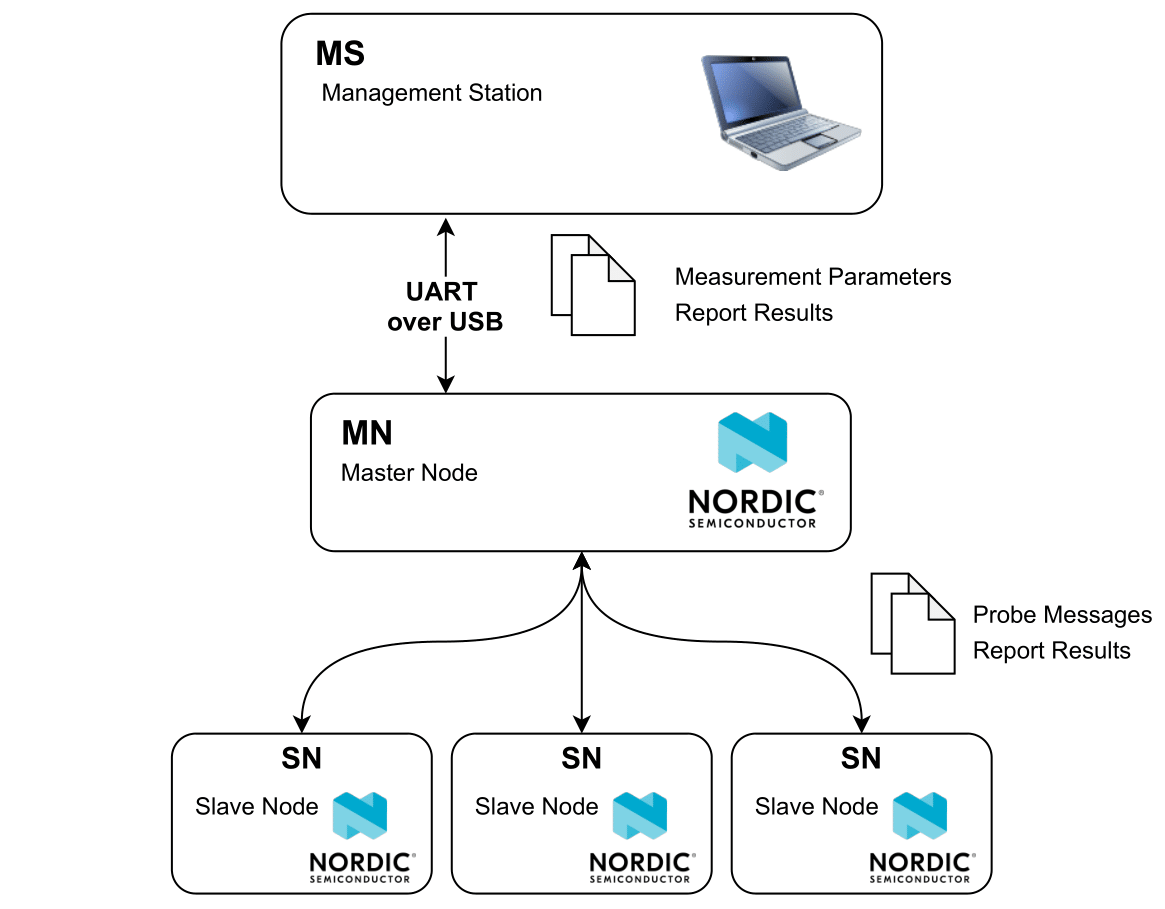
\includegraphics[width=0.8\textwidth]{Konzeptschema_P2P.png}
	\caption{Konzeptschema P2P Testinfrastruktur}
	\label{fig:KonzeptschemaP2P}
\end{figure}

Das in Abbildung \ref{fig:KonzeptschemaP2P} gezeigte Konzept besteht aus einer Managment Station, einem Master- und mehreren Slave Nodes. Über die Management Station können Messresultate angezeigt, sowie Messparameter eingestellt werden. Als Ausgangspunkt zur Messung dient der MN (Master Node). Er koordiniert den Messablauf und sendet \textit{Probe Packets} an alle SN (Slave Nodes). Diese Protokollieren die Anzahl empfangener \textit{Probe Packets} und melden ihre Messresultate an den MN zurück. Nach Empfang aller Resultate leitet der MN alle Messergebnisse an die MS weiter. Dort werden dem Benutzer die Messdaten dargestellt. Details zum Ablauf sind in Abschnitt \ref{sec:SoftundFirmware} aufgeführt. Eine mögliche Anwendung der Testinfrastruktur wird im folgenden Abschnitt \ref{sec:TestszenarienP2P} beschrieben.  

\subsection{Testszenarien}\label{sec:TestszenarienP2P}

Die P2P Testinfrastruktur ist als einfach zu bedienendes Tool konzipiert. Es kann eingesetzt werden um den Aufbau von PAN-Netzwerken zu optimieren. Mithilfe des Tools können zu Beispiel die Standorte der Teilnehmer eines Zigbee, Thread oder Bluetooth Mesh Netzwerks optimal gewählt werden. Zudem lassen sich während eines Messvorgangs gezielt Störungen in ein solches Netzwerk einbringen. Dadurch können die Netzwerke auf Störsicherheit geprüft werden. 



\subsection{Messaufbau}\label{sec:Messaufbau}

Bei der verwendeten Hardware handelt es sich um nRF52840 Mikrocontroller (siehe Abschnitt \ref{sec:HardwarePlattform}). Als Master dient das Development-Kit (DK), welches über eine USB-Buchse verfügt. Als Slaves kommen sowhl DKs als auch die USB-Dongle Variante in Frage. Letztere sind einfacher unterzubringen und werden in diesem Messaufbau bevorzugt. Um die Erhaltenen Daten auswerten zu können geschieht die Visualisierung mittels einem Laptop oder PC. Dieser muss mit der USB Buchse des Masters verbunden werden und die entsprechende Auswertesoftware gestartet sein. Im Folgenden Abschnitt wird die Inbetriebnahme und Bedienung der P2P-Testinfrastruktur genauer beschrieben. 

\begin{figure} [H]
	\centering
	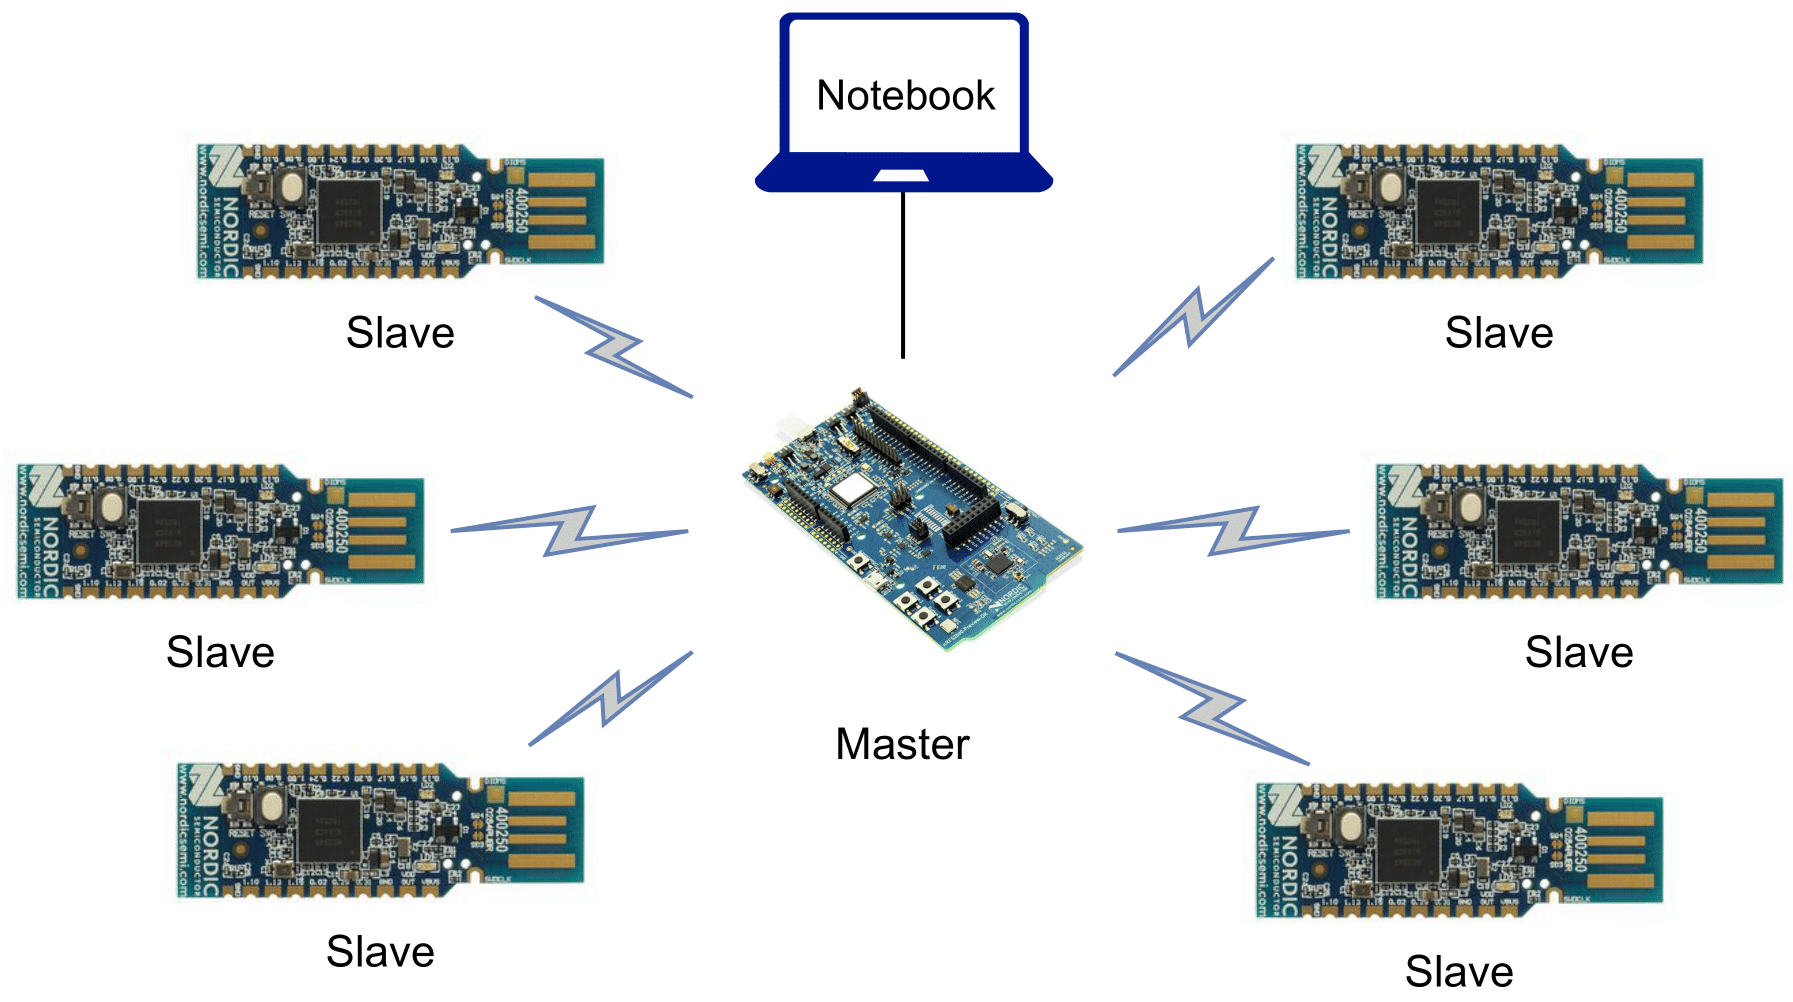
\includegraphics[width=0.8\textwidth]{Messaufbau_P2P.png}
	\caption{Messaufbau P2P Testinfrastruktur}
	\label{fig:MessaufbauP2P}
\end{figure}

Abbildung \ref{fig:MessaufbauP2P} zeigt den Messaufbau der P2P-Testinfrastruktur. Der Master kann mittels Laptop mobil gehalten werden um so den optimalen Standort des Masters anzupeilen. 


\newpage
\section{Inbetriebnahme und Bedienung}\label{sec:InbetriebnahmeBedienungP2P}


Zur Inbetriebnahme müssen folgende Voraussetzungen erfüllt werden: 

\begin{itemize}
	\item 1x nRF52840 DK (Master) und 1x nRF52840 DK / Dongle (Slave)
	\item Laptop mit folgender Software:
	\begin{itemize}
		\item Python 3.x
		\item nrfutil (pip install nrfutil), zum Flashen der nRF52840. 
		\item Django Framework, für Webserver
		\item Browser, zur Darstellung der Weboberfläche
	\end{itemize}
\end{itemize}

\todo[inline]{Robin: Was fehlt für Webserver?.}

Eine Anleitung und der Sourcecode sind im Internet verfügbar \cite{github_p6_software_p2p_2020}. Um den Master und Slaves vorzubereiten sind die beiden mit der entsprechenden Firmware zu laden. Anschliessend können die Slaves im Raum platziert und der Master am Laptop eingesteckt werden.  

\todo[inline]{Robin: wie weiter mit Webserver?}

\subsection{Schritt - Webserver Starten}\label{sec:SchrittWebserverStarten}
Der Webserver wurde mit eine Windows Umgebung entwickelt und getestet. Die folgende Anleitung funktioniert nur mit einer Windows Maschine. Für die Verwendung mit Linux oder MacOS sind auf der Hompage von Django Anleitungen verfügbar.
Bevor der Webserver gestartet werden kann, muss der Source-Code vom \href{https://github.com/Rouben94/P6_Software}{Github-Repository\footnotemark[\value{footnote}]} geklont werden. Auf der Ordnerebene \textbf{P6\_Software\textbackslash P2P\textbackslash Webserver\textbackslash p2p\_webserver} müssen folgende cmd Befehle ausgeführt werden.
\footnotetext{\url{https://github.com/Rouben94/P6_Software} \cite{anklin_bobst_horath_rouben94p6_software_nodate}}

\begin{lstlisting}[style=DOS]
Microsoft Windows [Version 10.0.18363.1016]
(c) 2019 Microsoft Corporation. Alle Rechte vorbehalten.

C:\Users\GitHub\P6_Software\P2P\Webserver\p2p_webserver> .\myvenv\Scripts\activate
(myvenv) C:\Users\GitHub\P6_Software\P2P\Webserver\p2p_webserver> python .\manage.py runserver
Performing system checks...
	
System check identified no issues (0 silenced).
August 20, 2020 - 22:01:13
Django version 3.0.8, using settings 'p2p_site.settings'
Starting development server at http://127.0.0.1:8000/   
Quit the server with CTRL-BREAK.
\end{lstlisting}

Nachdem ist der Webserver gestartet und kann unter der Adresse \textbf{http://127.0.0.1:8000/} erreicht werden.

\subsection{Schritt - Verbindungsaufbau}\label{sec:SchrittVerbindungsaufbau}

\begin{figure} [H]
	\centering
	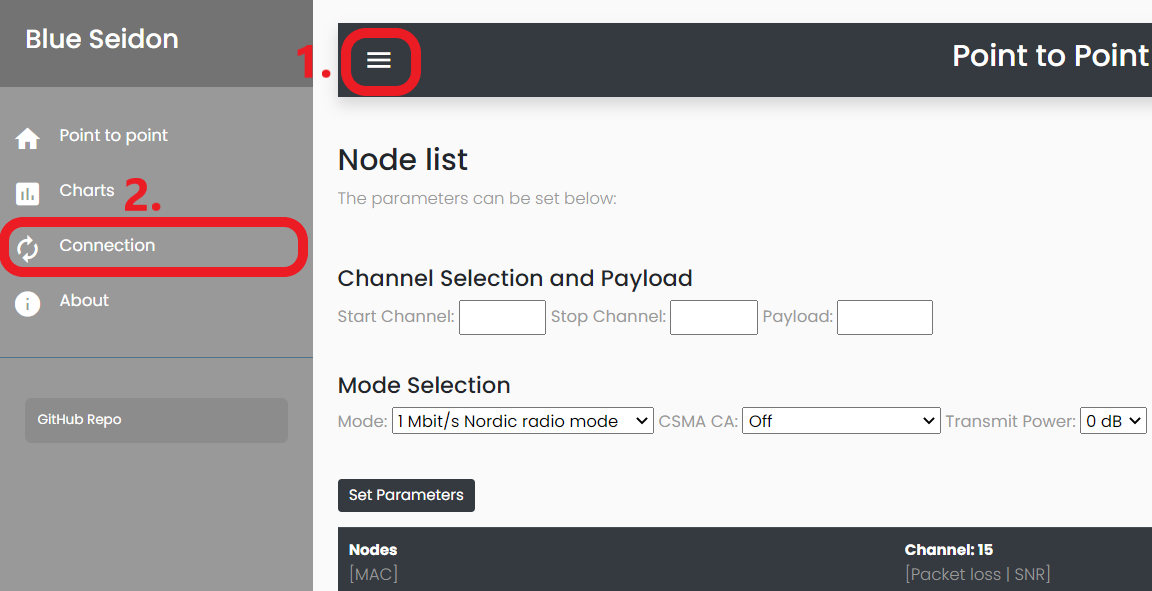
\includegraphics[width=\textwidth]{Webserver_nodelist_ausgeklappt.png}
	\caption{Webserver Nodelist View ausgeklappt}
	\label{fig:WebserverNodelistViewausgeklappt}
\end{figure}

\begin{figure} [H]
	\centering
	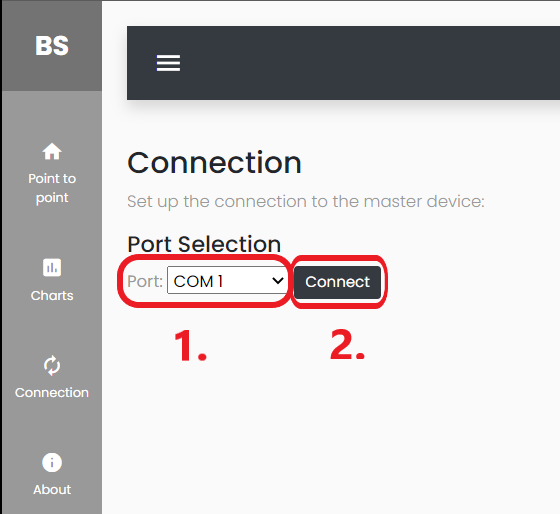
\includegraphics[width=\textwidth]{Webserver_Connection.png}
	\caption{Webserver Connection View}
	\label{fig:WebserverConnectionView}
\end{figure}


\subsection{Schritt - Parameter Einstellen}\label{sec:SchrittParameterEinstellen}
\begin{figure} [H]
	\centering
	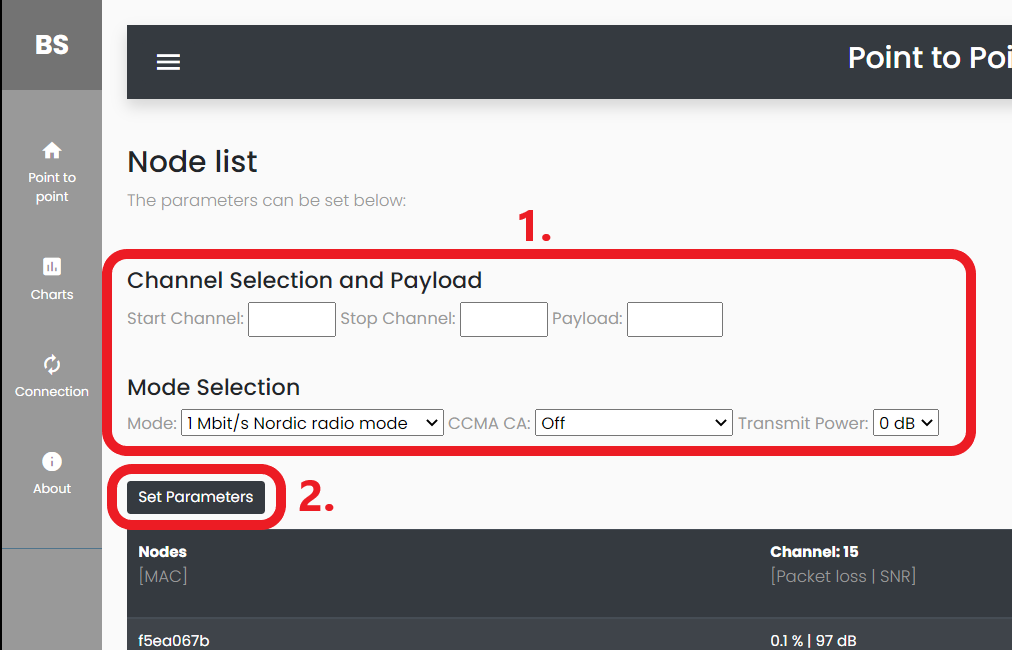
\includegraphics[width=\textwidth]{Webserver_Nodelist.png}
	\caption{Webserver Nodelist View}
	\label{fig:WebserverNodelistView}
\end{figure}

\subsection{Schritt - Channel Vergleichen}\label{sec:SchrittChannelVergleichen}
\begin{figure} [H]
	\centering
	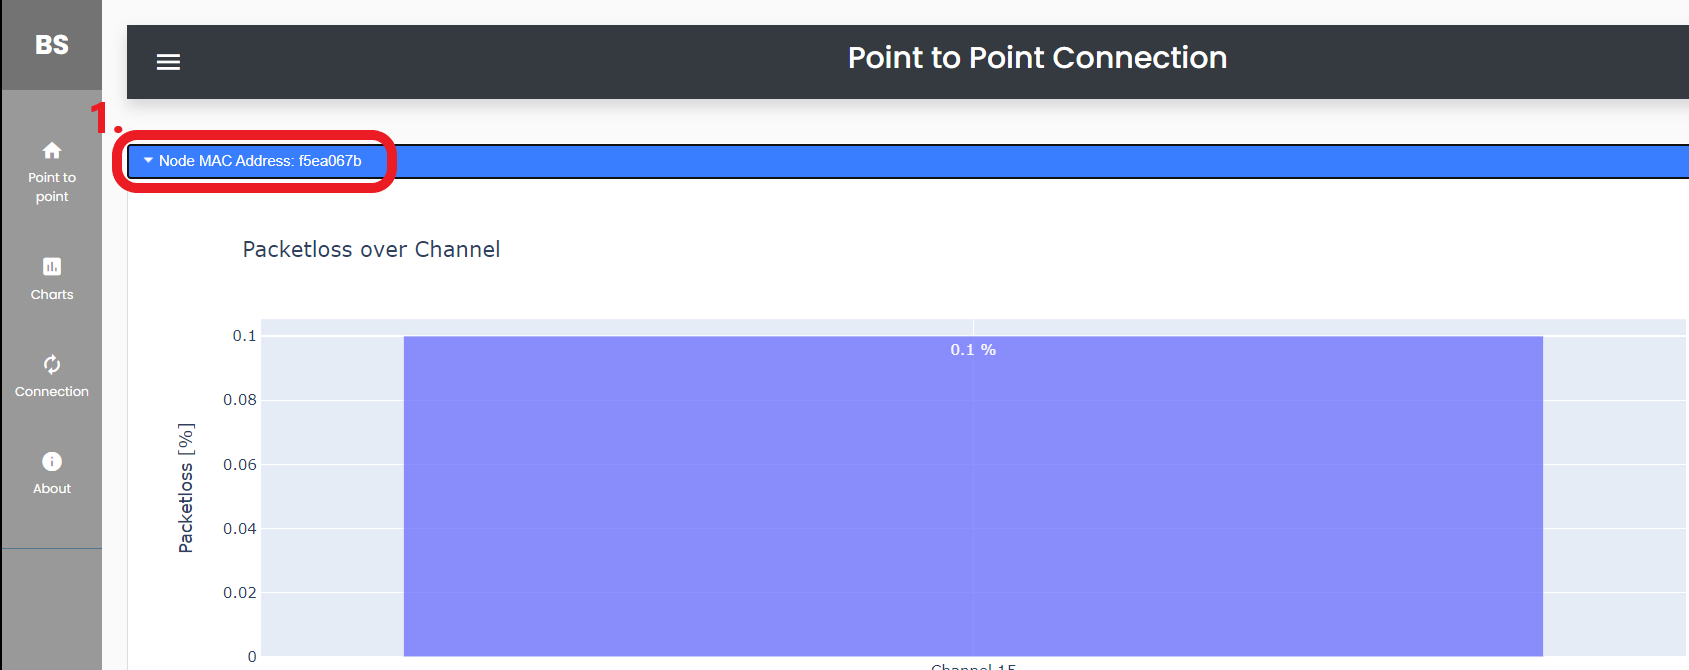
\includegraphics[width=\textwidth]{Webserver_Chart.png}
	\caption{Webserver Chart View}
	\label{fig:WebserverChartView}
\end{figure}



\newpage
\section{Soft- und Firmware}\label{sec:P2PSoft-undFirmware}

\subsection{Soft- und Firmware}\label{sec:SoftundFirmware}

Die Software ist als zeit-diskrete Schrittkette aufgebaut. Jeder Schritt ist über ein fixes Zeitfenster definiert, wodurch der Ablauf rein zeitabhängig vorgegeben ist. Damit alle Teilnehmer synchron ihre Schrittketten abarbeiten, muss mithilfe einer Zeitsynchronisation auf den Master der exakte Startzeitpunkt kommuniziert werden. Unabhängig vom Zustand des aktiven Schrittes, darf dieser sein Zeitfenster nicht überschreiten, ansonsten fällt die Schrittkette ausser Takt. 

\begin{figure} [H]
	\centering
	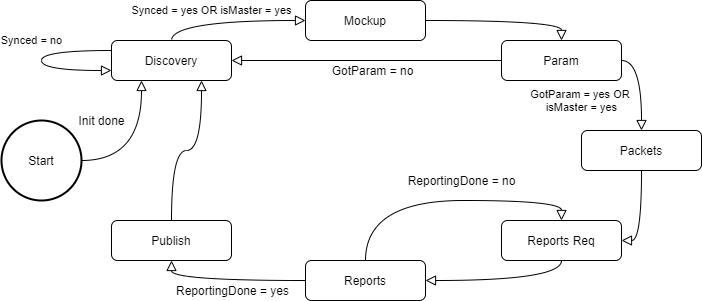
\includegraphics[width=1.0\textwidth]{Software_Flowgraph_P2P.png}
	\caption{Schrittkette P2P Testinfrastruktur}
	\label{fig:FlowgraphP2P}
\end{figure}

Abbildung \ref{fig:FlowgraphP2P} zeigt die Schrittkette für den Master, sowie für die Slave-Nodes. Der Ablauf zeigt die Schritte, sowie die Bedingungen der Transitionen zwischen den Schritten. Jedoch muss beachtet werden das jeder Schritt immer eine bestimmte Zeit aktiv bleibt. Somit ist ersichtlich das der \textit{Packets-State} nach Ablauf seines Zeitfensters immer zum \textit{ReportsReq-State} führt. Wobei der Wechsel nach dem \textit{Discovery-State} von verschiedenen Bedingungen abhängig ist. \\

Die Funktion der Schritte wird im Folgenden grob beschrieben. Zur genauen Untersuchung ist der Source Code unter \cite{github_p6_software_p2p_2020} verfügbar.  \\

\begin{itemize}
	\item \textbf{\textit{Discovery:}} Der Master verteilt die Zeitsynchronisation an die Slaves. Die Slaves synchronisieren sich auf das Signal des Masters auf, sofern sie in seiner Reichweite liegen. Hat ein Slave sich nicht Synchronisieren können verweilt dieser im \textit{Discovery-State}. Der Master darf immer zum nächsten Schritt voranschreiten. 
	\item \textbf{\textit{Mockup:}} Der Master wartet auf eine Antwort der einzelnen Slaves. Jeder Slave generiert einen zufälligen Timeslot um sich beim Master anzumelden. Der Master führt alle Slaves, welche sich gemeldet haben in einer Liste auf. Ist diese Liste leer (hat sich kein Slave gemeldet), so wird der Master zum \textit{Discovery State} zurückkehren. Ist ein Slave bereits beim Master angemeldet, so muss sich dieser nicht erneut anmelden. 
	\item \textbf{\textit{Param:}} Der Master versendet die Packets-Parameter (Mode, StartChannel, StopChannel, etc) auf welchen er die Probe-Packets versendet. Erhält ein Slave keine Daten so kehrt er in den \textit{Discovery-State} zurück. 
	\item \textbf{\textit{Packets:}} Der Master versendet \textit{Probe Packets} auf den zuvor Kommunizierten Einstellungen. Die Slaves empfangen diese Daten und zählen die Anzahl erfolgreich empfangener Pakete und erfassen weitere Messdaten. 
	\item  \textbf{\textit{Reports Req:}} Nach dem ausmessen beginnt der Master mit dem einsammeln der einzelnen Slave Reports. Dazu sendet er an jeden Slave in seiner Liste (aus dem \textit{Mockup-State}) Report-Anfragen, sogenannte \textit{Reports-Requests}. Die Slaves warten auf einen \textit{Report Request} vom Master. 
	\item  \textbf{\textit{Reports:}} Der Slave, welcher den Request bekommen hat, sendet seinen Report zum Master. Dies muss innerhalb einer gewissen Zeit erfolgen. Sendet ein Slave nach einer gewissen Anzahl von Versuchen keine Reports, wo wird er aus der Liste der gemeldeten Slaves entfernt. Sobald der Master alle Reports von allen Slaves empfangen hat, meldet er über eine spezielle \textit{Reports-Request-Message} an alle Slaves, dass das Reporting beendet ist.
	\item  \textbf{\textit{Publish:}} Im \textit{Publishing-State} hat der Master Zeit die Daten an die Übergeordnete stelle zu Übermitteln (USB-UART). Die Slaves können in diesem State Energie Sparen. Alle Teilnehmer beginnen wieder im \textit{Discovery-State}, wo sie sich neu Synchronisieren. 
\end{itemize}


\subsection{Low Level Radio Driver}\label{sec:LowLevelRadioDriver}

Die Kommunikation über das Radio-Interface wurde mittels einem eigens entwickeltem Radio-Driver, speziell für die nRF52 / nRF53 SOCs ermöglicht. Dieser stellt die nötigen Funktionen für die P2P Testinfrastruktur zur Verfügung. Zum Beispiel kann die Mode- und Kanalwahl sowie das Senden und Empfangen von Daten mittels simplen Kommandos erfolgen. Zur Entwicklung diente das \textit{Radio Test Example} \cite{nrf_connect_sdk_radio_test_example_2020} als Vorlage. Der Radio-Driver steuert mithilfe der \textit{NRF-HAL Radio Library} oder über direkten Zugriff auf die Peripherie-Register das Radio-Interface an.

\begin{figure} [H]
	\centering
	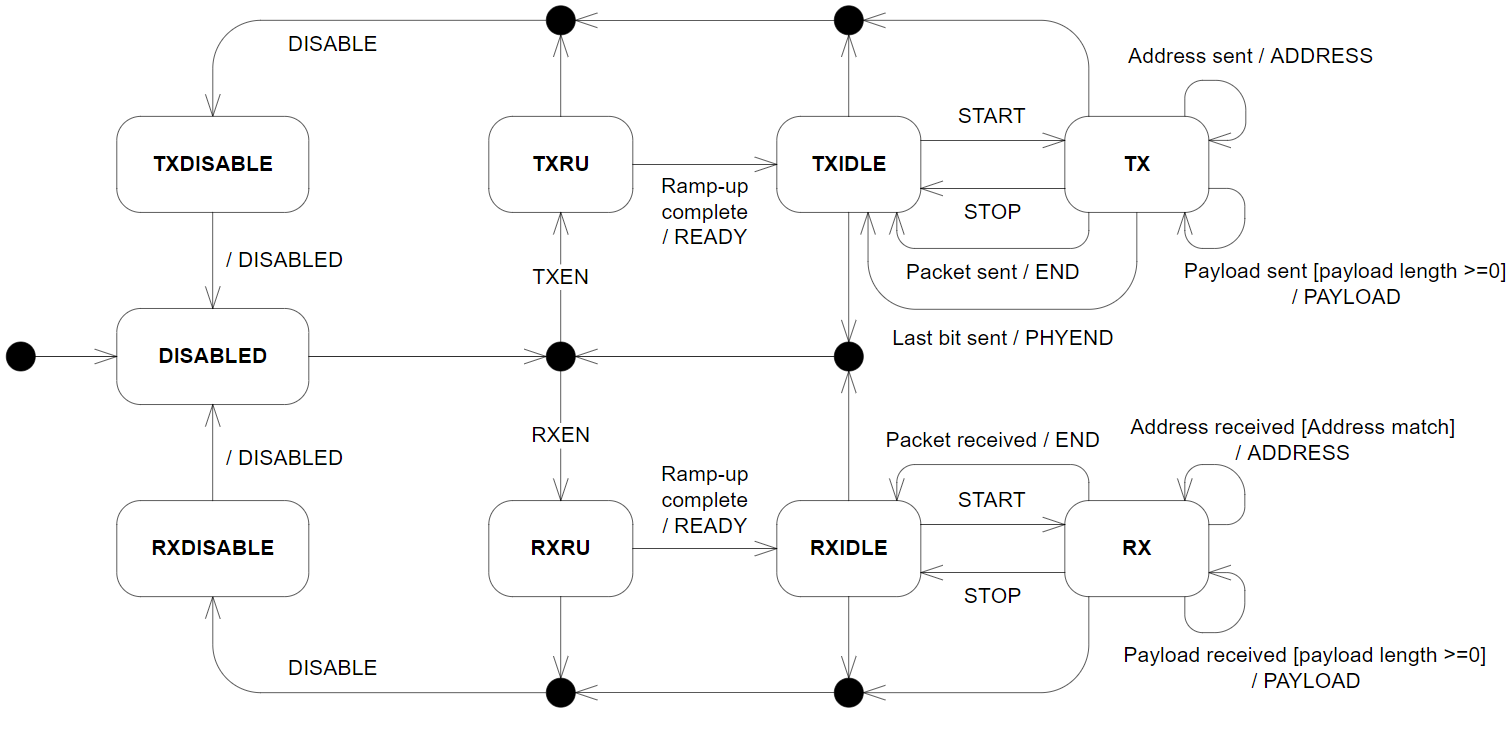
\includegraphics[width=1.0\textwidth]{nRF52840_Radio_states.png}
	\caption{Radio States \cite{nordic_semi_nrf_infocenter_radio_states_2020}}
	\label{fig:RadioStatesP2P}
\end{figure}

Die Radio Hardware der nRF52 und nRF53 SOCs verfügt über verschiedene Zustände (siehe Abbildung \ref{fig:RadioStatesP2P}). Abhängig von der gewünschten Operation (Senden oder Empfangen), werden die States abgearbeitet. Um Energie zu sparen wird nach Abschluss der gewünschten Tätigkeit immer in den Disabled-State gewechselt. Zusätzlich erfolgt das Benachrichtigen des Radio Drivers von der Hardware mittels Interrupts, wodurch der Energieverbrauch zusätzlich minimiert wird.

\begin{figure} [H]
	\centering
	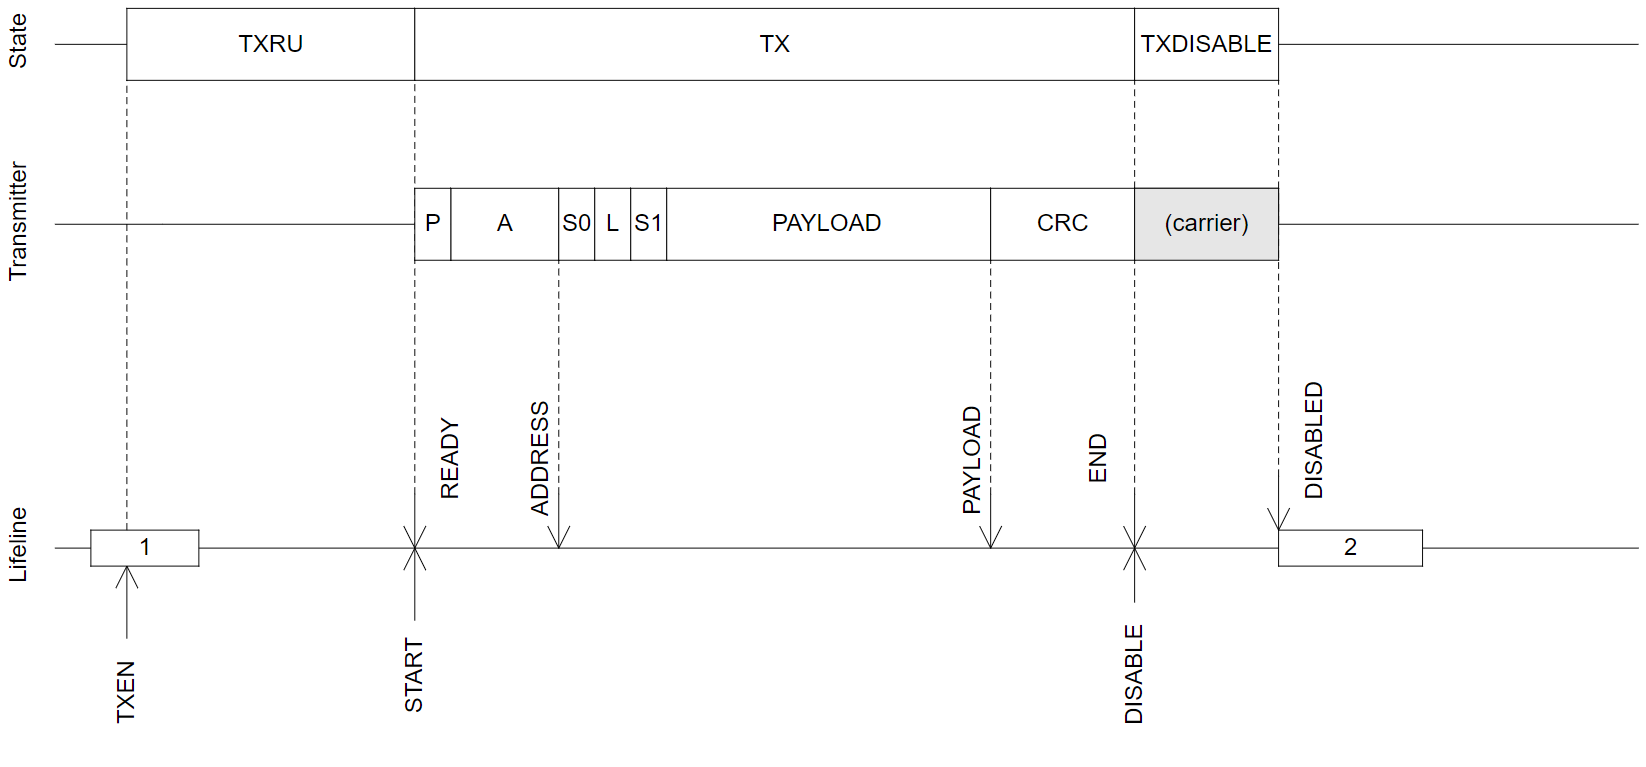
\includegraphics[width=1.0\textwidth]{nRF52840_Radio_Transmit_Sequence_with_Shorts.png}
	\caption{Sende-Ablauf mit Verknüpfungen \cite{nordic_semi_nrf_infocenter_radio_transmit_sequence_2020}}
	\label{fig:RadioTransmitSequP2P}
\end{figure}

Abbildung \ref{fig:RadioTransmitSequP2P} zeigt den Ablauf beim Senden eines Pakets. Die zu sendenden Daten (Payload) müssen vorgängig im RAM vorliegen. Anschliessend wird der Packet Pointer des Radio-Interface auf die entsprechende Speicher-Adresse eingestellt. Zu beachten gilt es das im ersten Byte die Länge der Payload angegeben sein muss. Diese wird vom Radio Driver automatisch ergänzt. Zusätzlich kann ein Adress-Feld den Sende-Daten mitgegeben werden. Nach dem vollständigen Konfigurieren des Radio-Interface wird das Senden durch den Befehl TXEN initiiert. Mithilfe von Verknüpfungen (Shorts) wird nach dem Ready-Event automatisch der Start-Task ausgelöst. Das Senden läuft also nach dem Initiieren vollautomatisch ab. Der Radio-Driver wartet lediglich auf das auslösen des Disabled-Events. Das Senden ist erfolgreich abgeschlossen und der Funktionsaufruf kehrt zum Hauptprogramm zurück. Das Senden mittels CCA wird im \textit{IEEE802.15.4-Mode} unterstützt. Dazu wird vor dem Senden der Kanal abgehört um Kollisionen zu vermeiden. Mittels dem RXEN Befehl wird der CCAStart-Task aktiv. Dieser führt abhängig vom Konfigurierten CCA-Modus eine Prüfung des Kanals durch. Ist der Kanal nicht belegt wird ein CCAIdle-Event generiert, welcher mittels Verknüpfung automatisch den TXEN-Task Startet (siehe Abbildung \ref{fig:CCAIDLEP2P}). Sendet ein andere Teilnehmer momentan auf dem Kanal wird ein CCABusy-Event generiert, welcher ebenfalls den Disable-Taks ausführt (siehe Abbildung \ref{fig:CCABUSYP2P}). Somit Enden beide Varianten (Idle und Busy) im Disabled-State, wobei beim einen keine Daten gesendet werden konnten. \cite{nordic_semi_nrf_infocenter_radio_transmit_sequence_2020}

\begin{figure}[!htbp]
	\begin{minipage}{0.49\textwidth}
		\centering
		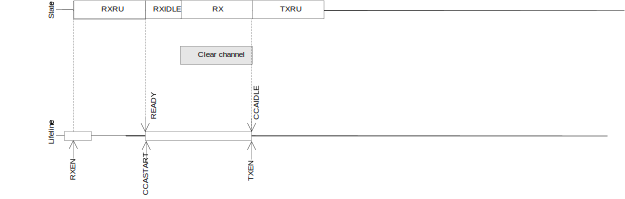
\includegraphics[width=\textwidth]{cca.png}
		\caption[Sende-Ablauf mit CCA Idle]{CCA Prüfung (Idle Event) \cite{nordic_semi_nrf_infocenter_radio_ieee_operation_2020}}
		\label{fig:CCAIDLEP2P}
	\end{minipage}
	\begin{minipage}{0.49\textwidth}
		\centering
		\includegraphics[width=\textwidth]{cca_busy.png}
		\caption[Sende-Ablauf mit CCA Busy]{CCA Prüfung (Busy Event) \cite{nordic_semi_nrf_infocenter_radio_ieee_operation_2020}}
		\label{fig:CCABUSYP2P}
	\end{minipage}
\end{figure}

\begin{figure} [H]
	\centering
	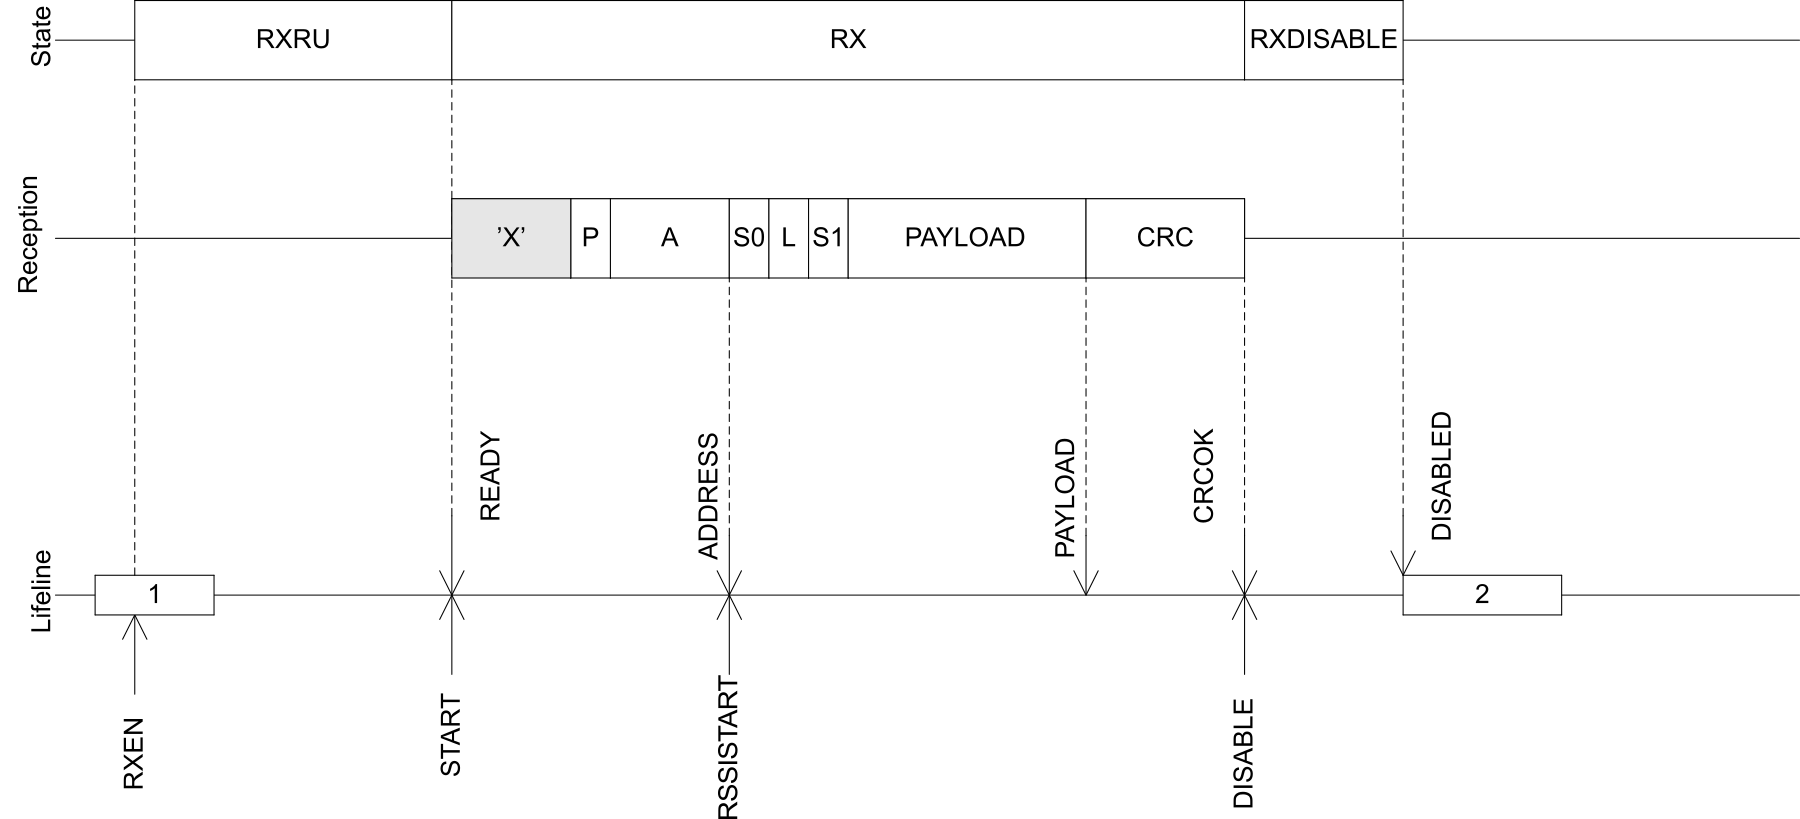
\includegraphics[width=1.0\textwidth]{nRF52840_Radio_Receive_Sequence_with_Shorts.png}
	\caption{Empfangs-Ablauf mit Verknüpfungen \cite{nordic_semi_nrf_infocenter_radio_receive_sequence_2020}}
	\label{fig:RadioReceiveSequP2P}
\end{figure}


Der Ablauf zum Empfangen eines Pakets wird in Abbildung \ref{fig:RadioReceiveSequP2P} dargestellt. Grundsätzlich ist der Ablauf gleich Aufgebaut wie beim Senden von einem Paket. Nach Initiieren mittels dem RXEN-Befehl fährt der Empfänger hoch und wartet auf den Empfang eines Pakets. Nach eingehen einer Preamble-Sequenz wird das Address-Feld geprüft. Dieses kann vorgängig festgelegt werden um nur Pakete mit übereinstimmender Adresse zu empfangen. Bei allen BLE-Modes erfolgt die Prüfung auf Hardware-Ebene (ohne Interaktion der CPU) ab. Beim \textit{IEEE802.15.4-Mode} steht dieses Feature nicht zur Verfügung. Das vergleichen des Adress-Feldes muss der Radio-Driver selbst übernehmen. Um die Signalstärke (RSSI) vom eingehenden Paket zu messen, wird eine Verknüpfung zwischen dem \textit{Address-Event} und dem \textit{RSSIStart-Task} aktiviert. Nach erfolgreichem Prüfen der CRC Checksumme wird mittels einer Verknüpfung des CRCOK-Event der Disable-Task ausgeführt. Beim Empfangen eines Pakets wartet der Radio-Driver während eines gewissen Timeouts auf den Disabled-Event. Die Empfangsfunktion gibt die Restzeit des Timeouts in Millisekunden zurück, wodurch sich ein erfolgreiches Empfangen prüfen lässt. Das Bufferhandling übernimmt der Radio-Driver und erwartet beim Senden und Empfangen von Daten eine vordefinierte \textit{Radio-Packet-Structure}. Zu beachten gilt es das die Daten erst nach dem End-Event  vollständig abgearbeitet wurden, da der Zugriff von der Hardware über DMA erfolgt. Ebenfalls wurde festgestellt das beim wechseln auf oder von dem \textit{IEEE802.15.4-Mode} der Kanalwechsel vor dem Modewechsel erfolgen muss. Ansonsten werden keine Pakete empfangen. \cite{nordic_semi_nrf_infocenter_radio_receive_sequence_2020}


\subsection{Broadcasting Collisions Probability}\label{sec:BroadcastingCollissionsProbability}

Kollisionen entstehen wenn mehrere Teilnehmer gleichzeitig auf dem selben Kanal (Frequenz) senden. Dabei stören sich die beiden Sender und es kann sein das der Empfänger keine Daten empfangen kann. Dies ist leider nicht immer zu vermeiden, zum Beispiel wenn sich mehrere Teilnehmer neu mit dem Netz verbinden möchten. Im Fall der P2P-Testinfrastruktur entsteht ein solcher Fall im Mockup-State. Hier soll sich jeder Slave, welcher dem Master noch unbekannt ist, auf die Discovery-Anfrage des Masters melden. Die Lösung ist das jeder Slave einen zufälligen Zeitpunkt zum Antworten auswählt. Doch wie lange muss das Zeitfenster sein in welchem ein Slave einen Zeitpunkt zufällig auswählen darf? \\

Angenommen es gibt $N$ Teilnehmer, welche $t_a$ Sekunden brauchen um eine Antwort zu Senden. Zusätzlich existieren $N_{ch}$ verschiedene Kanäle auf welchen die Teilnehmer antworten können. Die Wahrscheinlichkeit das sich zwei Sender nicht überlappen $P_{miss}$ im Zeitfenster $t_I$ Sekunden lässt sich gemäss Formel \ref{eq:BroadcastingMissProbability} bestimmen. \cite{rk_how_to_deal_with_broadcasting_collision_2020}

\begin{equation}\label{eq:BroadcastingMissProbability}
P_{miss} = (1- \frac{2 \cdot t_a}{N_{ch}} \cdot t_I)^{N-1}
\end{equation}

Die folgenden Werte wurden zur Berechnung des Zeitfensters im Mockup-State verwendet:

\begin{itemize}
	\item $N = 50$
	\item $t_a = 5ms$
	\item $N_{ch} = 3$
	\item $t_I = 1.2s$	
\end{itemize} 

Somit liegt die Wahrscheinlichkeit das alle 50 Nodes sich verfehlen bei 85\%. 

\subsection{Zeitsynchronisation}\label{sec:ZeitsynchronisationP2P}

Die Zeitsynchronisation wurde mittels einer Offset Kompensation gelöst. Der Zeitgeber (Master) sendet seine Zeit (Timestamp) über einen Broadcast an alle Teilnehmer in der Umgebung. Die Slaves vergleichen den empfangene Master-Zeit mit ihrer lokalen Zeit und errechnen den Unterschied (Offset) zwischen dem Master-Timestamp und Slave-Timestamp. Somit können sie ihre Zeit mittels an die des Masters angleichen. Das Prinzip ist realtiv simpel birgt jedoch einige Ungenauigkeiten. Die Verzögerungszeit zwischen dem auslesen des Master-Timestamp bis zum empfangen und vergleichen mit dem Slave-Timestamp ist sehr relevant.  

\begin{figure} [H]
	\centering
	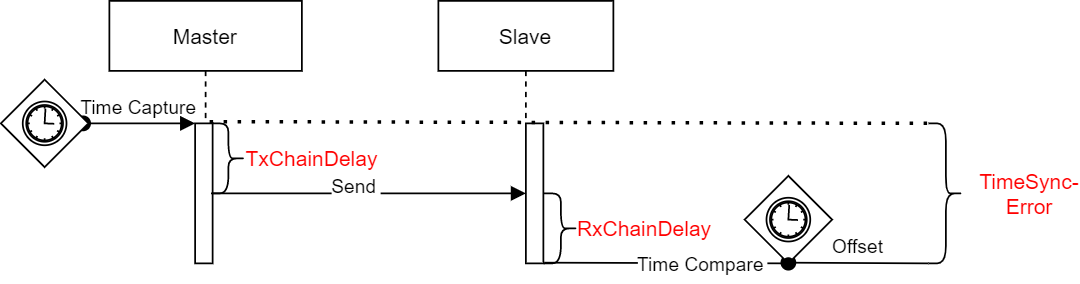
\includegraphics[width=1.0\textwidth]{Timesync_Basic.png}
	\caption{Zeitsynchronisation über Offset mit Fehler}
	\label{fig:TimesyncBasicwithErrorP2P}
\end{figure}

Wie in Abbildung \ref{fig:TimesyncBasicwithErrorP2P} ersichtlich entsteht beim Auslesen der Zeit bis zum Senden eine Verzögerung die TxChainDelay, sowie beim Empfänger die RxChainDelay. Das Ziel ist es diese Verzögerungen so gering wie möglich zu halten. 

\begin{figure} [H]
	\centering
	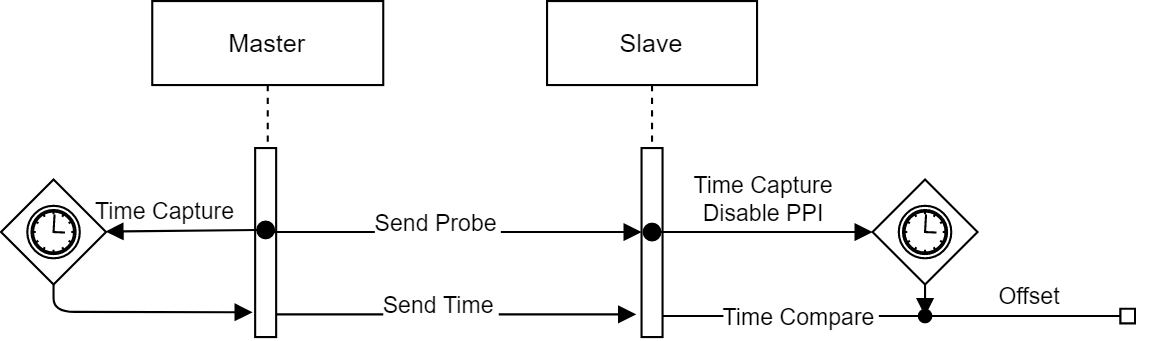
\includegraphics[width=1.0\textwidth]{Tiesync_Advanced.png}
	\caption{Zeitsynchronisation über Offset mit PPI}
	\label{fig:TimesyncwithPPIP2P}
\end{figure}

Die Lösung wird in Abbildung \ref{fig:TimesyncwithPPIP2P} gezeigt. Der nRF52840 SOC verfügt über ein PPI (Programmable peripheral interconnect). Mithilfe des PPI lassen sich verschiedene Events und Tasks direkt Verknüpfen, ohne das die CPU dabei involviert ist. Dies führt zu minimalen Verzögerung (ca. 1/16 us) zwischen Event und Task. Dazu wird der Event, dass ein Packet erfolgreich Gesendet wurde (Radio-End-Event), mit dem Task zum Erfassen des Synctimers (Synctimer-Capture-Task) verknüpft. Beim Slave wird der Event, dass ein Packet erfolgreich Empfangen wurde (Radio-CRCOK-Event), mit dem Task zum Erfassen des Synctimers (Synctimer-Capture-Task) verknüpft. Nach dem empfangen muss der Slave diesen PPI sofort deaktivieren, da ein direkt folgendes Paket ebenfalls ein Erfassen des Timers auslöst. Der Master wird nach deaktivieren des PPI mit einem Folge-Paket seine Master-Zeit dem Slave mitteilen, welche zum Zeitpunkt des Probe-Packets registriert wurde. Der Slave errechnet den Offset gemäss Formel \ref{eq:TimesyncOffsetSynctimeCalc} und die Synchronisierte-Zeit mit der Formel \ref{eq:TimesyncSynctimeCalc}. \cite{nordic_semi_nrf_infocenter_ppi_2020}

\begin{equation}\label{eq:TimesyncOffsetSynctimeCalc}
T_{Offset} =  T_{Master} - T_{Slave} 
\end{equation}

\begin{equation}\label{eq:TimesyncSynctimeCalc}
T_{Sync} =  T_{Slave} + T_{Offset} 
\end{equation}

Zur Verifikation der Zeitsynchronisation wurde ein Oszilloskop an jeweils einen GPIO-Pin am Master und einen am Slave angeschlossen. Auf dem Master und Slave wurden nacheinander Timer-Interrupts registriert, welche relativ zur synchronisierten Zeit auf dem Master und Slave genau gleichzeitig auslösen. Mithilfe eines PPI-Kanals wurde der Interrupt-Event auf den GPIO-Pin Verknüpft. Beim auslösen des Interrupts wird der Zustand des GPIO-Pins getoggelt. Somit wird die Abweichung Präzise auf dem Oszilloskop ersichtlich.

\begin{figure} [H]
	\centering
	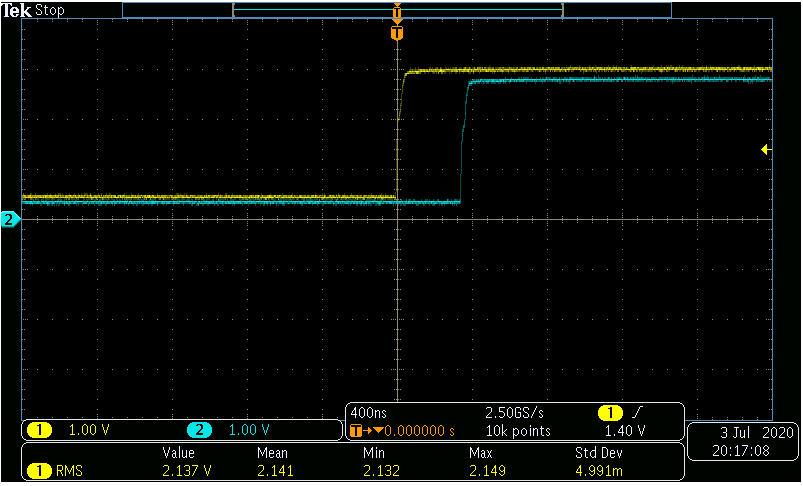
\includegraphics[width=1.0\textwidth]{Messungen Timesync (100ns 1200ns).png}
	\caption{Verifikation Zeitsynchronisation}
	\label{fig:TimesyncVerifikationP2P}
\end{figure}

Abbildung \ref{fig:TimesyncVerifikationP2P} zeigt den Signalverlauf der GPIOs vom Master (gelb) und Slave (blau). Anfänglich lagen die Abweichungen im Bereich von ca. 40us. Durch Wiederholungen der Messung konnte dieser Fehler als systematisch identifiziert werden. Mithilfe einer Korrektur um 40us konnte die Genauigkeit in den Bereich von 100ns bis 1200ns reduziert werden. Eine Abweichung der Zeitsynchronisation von ca. 1us sollte genügend genau sein um als gute Grundlage für die Statemachine aus Abschnitt \ref{sec:SoftundFirmware} zu dienen. 
 
 \newpage
\subsection{Webserver}\label{subsec:DjangoWebserver}
\subsubsection{Django}\label{subsubsec:Django}
Um die P2P-Testinfrastruktur bedienen zu können, wurde ein Django Webserver geschrieben. Django ist ein open-source Webframework, dass auf dem Model-View-Controller verfahren basiert und in der Programmiersprache Python geschrieben wurde. Das Framwork hat sein eigenes Benennungssystem für alle Funktionen und Komponenten. Zum Beispiel werde HTTP-Antworten als Views bezeichnet. Ein grosser Vorteil von Django ist die Administrationsseite. Die Admin-Seite ist Bestandteil des Projekts und dient dazu die Models zu verwalten. Models sind Objekte, die in einer Datenbank des Webservers gespeichert werden. Die gängigsten Datenbanksysteme, wie z.B. SQLLite sind in Django integriert und können einfach aktiviert oder bzw. implementiert werden. In der Tabelle \ref{table:FeaturesDjango} sind die wichtigsten Features von Django aufgelistet:

\begin{table}[H]
	\centering
	\begin{adjustbox}{width=1\textwidth}
		\begin{tabular}{@{}|l|l|l|@{}}
			\toprule
			\multicolumn{3}{|c|}{\textbf{Features}}                                        \\ \midrule
			Einfacher Syntax (Python) & Model-View-Controller      & Administrations Seite \\ \midrule
			Model-View-Controller     & Eigener Webserver          & Gängigste Datenbanken \\ \midrule
			HTTP Bibliothek           & Python Unit Test Framework & Models für Datenbank  \\ \bottomrule
		\end{tabular}
	\end{adjustbox}
	\caption{Features Django}
	\label{table:FeaturesDjango}
\end{table}

 \newpage
\subsubsection{Software Grundlagen}\label{subsubsec:SoftwareGrundlagen}
Bei einer gewöhnlichen datengesteuerten Webseite wartet die Webanwendung auf eine HTTP-Anfrage des Browsers. Wird ein Anfrage empfangen so bestimmt die Anwendung auf der Grundlage der URL, ob ein GET oder POST Event ausgelöst wird. Je nach Anfrage wird somit aus einer Datenbank gelesen oder es wird in die Datenbank geschrieben. Die Anwendung schickt danach eine Antwort an den Web-Browser, wobei häufig eine HTML-Seite erzeugt wird, um die Antwort darzustellen. Diese Schritte sind in Django, wie in der Abbildung \ref{fig:DjangoAblauf} aufgeführt,  in separaten Dateien zusammengefasst.
\begin{figure} [H]
	\centering
	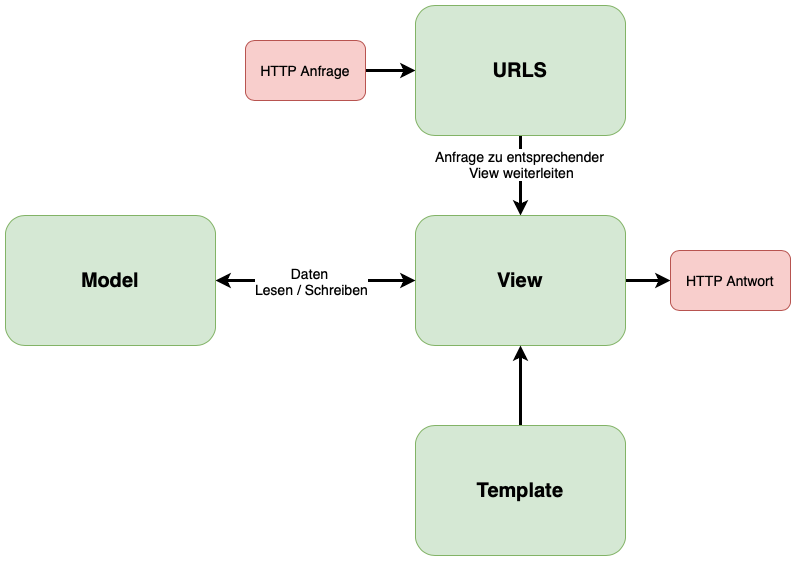
\includegraphics[width=0.76\textwidth]{Django Ablauf.png}
	\caption{Django Funktionen}
	\label{fig:DjangoAblauf}
\end{figure}

\paragraph{URLs: }\label{par:1URLs}
Die URL Datei leitet die Anfrage an die entsprechende View weiter. Damit dies gelingt wird ein URL-Mapper eingesetzt. Dieser dient dazu, die Anfrage so zu interpretieren, damit die richtige View aufgerufen wird. Zusätzlich erkennt der URL-Mapper Zeichenketten und Ziffern in der URL und kann diese abgleichen und anschliessend als Daten an die View-Funktion weitergeben.

\paragraph{Views: }\label{par:1Views}
Die View ist eine Request-Handler-Funktion, die HTTP Anfragen empfängt un zurückgibt. Die View kann über die Model Funktion auf Daten in der Datenbank zugreifen. Über die Template Funktion beschreibt die View schlussendlich, wie die HTTP-Antwort formatiert werden muss.

\paragraph{Models: }\label{par:1Models}
Ein Model ist ein Python Objekt, die die Struktur der Daten einer Anwendung definieren. Darüber hinaus stellt die Funktion die Mittel bereit, um die Daten in der Datenbank zu verwalten, wie z.B Hinzufügen, Löschen oder Ändern. Die Model Funktion ist somit die Schnittstelle zu der Datenbank.

\paragraph{Templates: }\label{par:1Templates}
Das Template ist eine Textdatei, in der die Struktur oder das Layout einer HTML-Seite definiert wird. Für die Struktur werden Platzhalter zur Darstellung des eigentlichen Inhalts  verwendet. Demnach kann die View-Funktion mit Hilfe vom Template eine dynamische HTML-Seite erzeugen und mit Daten von der Model-Funktion füllen.

\newpage
\subsubsection{Software Aufbau}\label{subsubsec:SoftwareAufbau}
Der Aufbau des Django Weberservers für die P2P-Testinfrastruktur ist in der Abbildung \ref{fig:FunktionenP2PWebserver} ersichtlich.
\begin{figure} [H]
	\centering
	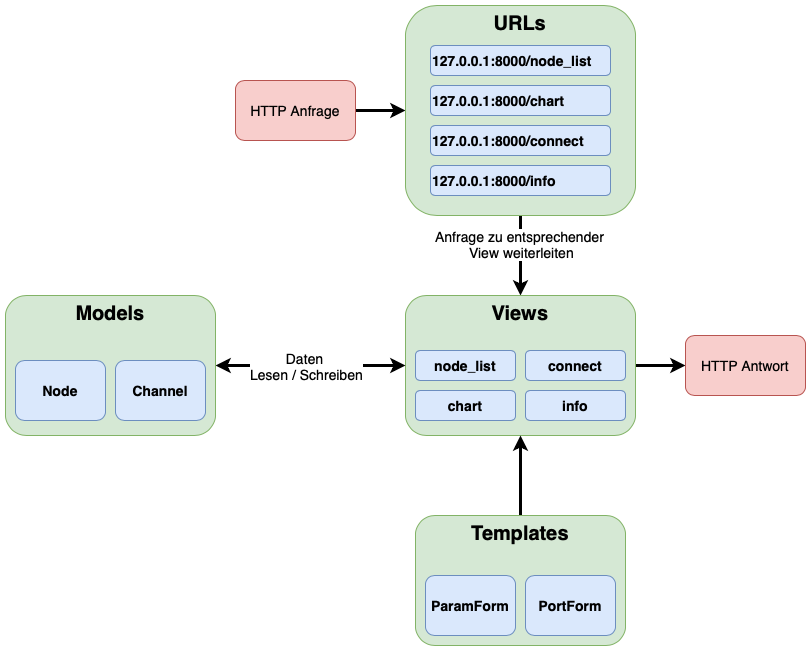
\includegraphics[width=0.9\textwidth]{DjangoSoftwaredoku.png}
	\caption{Funktionen P2P Webserver}
	\label{fig:FunktionenP2PWebserver}
\end{figure}


\paragraph{URLs: }\label{par:2URLs}
In der folgenden Tabelle sind alle URLs aufgelistet, welche verwendet wurden um auf die entsprechenden Views zu zeigen.
\begin{itemize}
	\item 127.0.0.1:8000/node\textunderscore list \hspace{2.5mm} referenziert auf die View node\textunderscore list
	\item 127.0.0.1:8000/chart \hspace{10mm} referenziert auf die View chart
	\item 127.0.0.1:8000/connect \hspace{6mm} referenziert auf die View connect
	\item 127.0.0.1:8000/info \hspace{12.5mm} referenziert auf die View info
\end{itemize} 

\vspace{5mm}
\paragraph{Views:}\label{par:2Views}
Es wurden vier Views im P2P-Webserver erstellt, die die Schnittstellen zu den Forms, den Models und der HTML-Dateien bilden:
\begin{itemize}
	\item Node\textunderscore list View
	\item Chart View
	\item Connect View
	\item Info View
\end{itemize} 
Die Bedienung der einzelnen Seiten wird im Kapitel \ref{sec:BedienungMessinfrastruktur} erläutert.

\newpage
\paragraph{Models: }\label{par:2Models}
Für die Speicherung der Daten vom NRF52 Master, sind zwei Objekte verfügbar: 
\begin{itemize}
	\item Objekt Node
	\item Objekt Channel
\end{itemize} 

\vspace{3mm}
Die zwei Objekte sind miteinander verknüpft. Wenn ein Node Objekt erstellt wird können die dazugehörigen Channel Informationen dazu erstellt werden. Dadurch ist eine klare Struktur gegeben. Über das Node Objekt können die verschiedenen Channel Informationen abgerufen werden. \\


Folgende Parameter können dem Objekt Node als Information mitgegeben werden:
\begin{itemize}
	\item MAC Adresse
\end{itemize} 

\vspace{3mm}
Folgende Parameter können dem Objekt Channel als Information mitgegeben werden:
\begin{itemize}
	\item Channel Nummer
	\item Signal to noise ratio
	\item Packetloss
	\item Node ID
\end{itemize}

\vspace{5mm}
\paragraph{Templates: }\label{par:2Templates}
Als Template wurden zwei verschiedene Django Forms erstellt. Eine Form ist eine Anordnung an Eingabefeldern, die frei bestimmt werden können. Die Drop Down Auswahlmöglichkeiten sind in der Tabelle \ref{table:TabelleAuswahlfelder} aufgelistet. \\

Für die Eingabe der Parameter, die auf dem P2P-Master eingestellt werden können, ist die Form ParamForm mit folgenden Eingabefeldern verfügbar:
\begin{itemize}
	\item Start Channel \hspace{5mm} -> Integer Feld
	\item Stop Channel \hspace{6mm} -> Integer Feld
	\item Size \hspace{22.3mm} -> Integer Feld
	\item Mode \hspace{19.5mm} -> Drop Down Auswahlfeld
	\item CCMA CA \hspace{10mm} -> Drop Down Auswahlfeld
	\item Tx Power \hspace{13mm} -> Drop Down Auswahlfeld
\end{itemize}

\vspace{3mm}
Für die Auswahl des Ports für die Serielle Verbindung zum Master, ist die Form PortForm mit folgenden Eingabefeldern verfügbar:
\begin{itemize}
	\item  Port \hspace{22mm} -> Drop Down Auswahlfeld
\end{itemize}

\begin{table}[H]
	\centering
	\begin{adjustbox}{width=1\textwidth}
		\begin{tabular}{@{}llll|l|l|l|@{}}
			\toprule
			\multicolumn{7}{|c|}{\textbf{Auswahlfelder}}                                                                                                                                                                                    \\ \midrule
			\multicolumn{1}{|c|}{\textbf{Auswahl Mode}}         & \multicolumn{1}{l|}{} & \multicolumn{1}{c|}{\textbf{Auswahl CCMA CA}} &  & \multicolumn{1}{c|}{\textbf{Auswahl Tx Power}} &  & \multicolumn{1}{c|}{\textbf{Auswahl Port}} \\ \cmidrule(r){1-1} \cmidrule(lr){3-3} \cmidrule(lr){5-5} \cmidrule(l){7-7} 
			\multicolumn{1}{|l|}{1 Mbit/s Nordic radio mode}    & \multicolumn{1}{l|}{} & \multicolumn{1}{l|}{Off}                      &  & 0 dB                                           &  & Disconnect                                 \\ \cmidrule(r){1-1} \cmidrule(lr){3-3} \cmidrule(lr){5-5} \cmidrule(l){7-7} 
			\multicolumn{1}{|l|}{2 Mbit/s Nordic radio mode}    & \multicolumn{1}{l|}{} & \multicolumn{1}{l|}{Ed Mode}                  &  & 1 dB                                           &  & COM 1                                      \\ \cmidrule(r){1-1} \cmidrule(lr){3-3} \cmidrule(lr){5-5} \cmidrule(l){7-7} 
			\multicolumn{1}{|l|}{1 Mbit/s BLE}                  & \multicolumn{1}{l|}{} & \multicolumn{1}{l|}{Carrier Mode}             &  & 2 dB                                           &  & COM 2                                      \\ \cmidrule(r){1-1} \cmidrule(lr){3-3} \cmidrule(lr){5-5} \cmidrule(l){7-7} 
			\multicolumn{1}{|l|}{2 Mbit/s BLE}                  & \multicolumn{1}{l|}{} & \multicolumn{1}{l|}{Carrier and Ed Mode}      &  & 3 dB                                           &  & COM 3                                      \\ \cmidrule(r){1-1} \cmidrule(lr){3-3} \cmidrule(lr){5-5} \cmidrule(l){7-7} 
			\multicolumn{1}{|l|}{Long range 125 kbit/s TX}      & \multicolumn{1}{l|}{} & \multicolumn{1}{l|}{Carrier or Ed Mode}       &  & 4 dB                                           &  & COM 4                                      \\ \cmidrule(r){1-1} \cmidrule(lr){3-3} \cmidrule(lr){5-5} \cmidrule(l){7-7} 
			\multicolumn{1}{|l|}{Long range 500 kbit/s TX}      &                       &                                               &  & 5 dB                                           &  & COM 5                                      \\ \cmidrule(r){1-1} \cmidrule(lr){5-5} \cmidrule(l){7-7} 
			\multicolumn{1}{|l|}{IEEE 802.15.4-2006 250 kbit/s} &                       &                                               &  & 6 dB                                           &  & COM 6                                      \\ \cmidrule(r){1-1} \cmidrule(lr){5-5} \cmidrule(l){7-7} 
			&                       &                                               &  & 7 dB                                           &  & COM 7                                      \\ \cmidrule(lr){5-5} \cmidrule(l){7-7} 
			&                       &                                               &  & 8 dB                                           &  & \textbf{...}                               \\ \cmidrule(lr){5-5} \cmidrule(l){7-7} 
		\end{tabular}
	\end{adjustbox}
	\caption{Tabelle Auswahlfelder}
	\label{table:TabelleAuswahlfelder}
\end{table}

In der Abbildung \ref{fig:ParamForm} und \ref{fig:PortForm} sind die Eingabe Forms ersichtlich. Die Daten werden mit einem Button, der ein HTTP-POST Ereignis auslöst, an die entsprechende View weitergeleitet.

\begin{figure} [H]
	\centering
	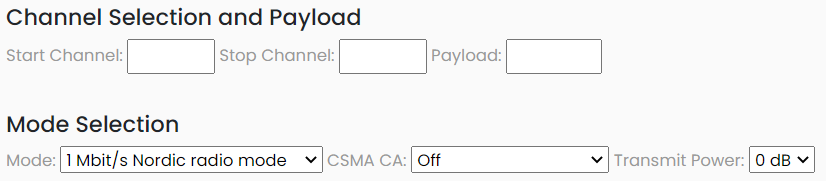
\includegraphics[width=\textwidth]{ParamForm.png}
	\caption{Parameter Form}
	\label{fig:ParamForm}
\end{figure}


\begin{figure} [H]
	\centering
	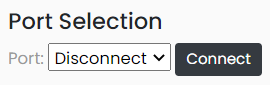
\includegraphics[width=0.5\textwidth]{PortForm.png}
	\caption{Port Form}
	\label{fig:PortForm}
\end{figure}

\newpage

\paragraph{Serielle Kommunikation: }\label{par:SerielleKommunikation}
Die Serielle Kommunikation wird mit Hilfe der Python Bibliothek PySerial aufgebaut. Auf der P2P-Webserver Seite Connect, kann der Port ausgewählt werden, an dem der P2P-Master angeschlossen ist. Sobald die Verbindung zum Master aufgebaut ist, wird ein seperater Python Thread gestartet. In diesem Thread wird in einem while-loop das Serielle Interface permanent ausgelesen. Sobald der Master einen neuen Mess-Report schickt, wird dieser ausgewertet und es werden Node und Channel Objekte anhand der Reports erstellt. In der Abbildung \ref{fig:AblaufDjangoSerial} ist der Ablauf ersichtlich.

Die erhaltenen Daten werden in der View Node\textunderscore List in einer Dynamischen Tabelle, die jede Sekunde Aktualisiert wird angezeigt. Zudem ist in der View Chart ein Visualisierung der Daten ersichtlich. Die Messergebnisse werden mit Hilfe der Bibliothek PlotLy dargestellt. \\

\begin{figure} [H]
	\centering
	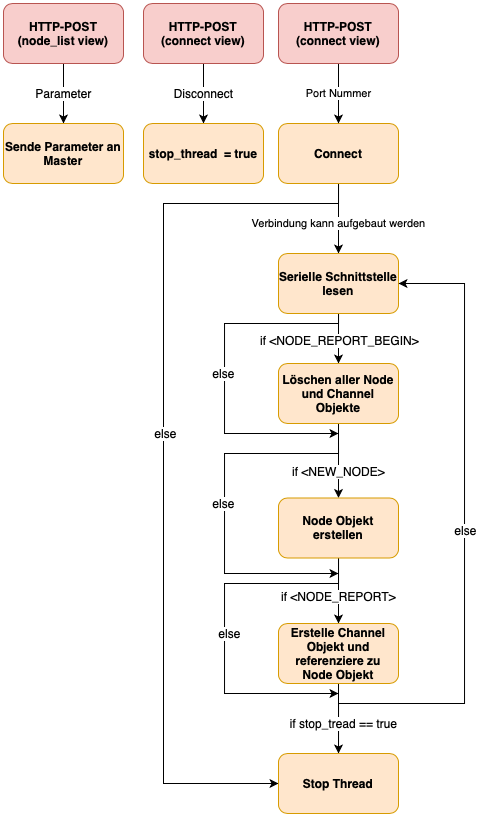
\includegraphics[width=0.63\textwidth]{Ablauf Django Serial.png}
	\caption{Ablauf Django Serial}
	\label{fig:AblaufDjangoSerial}
\end{figure}


\section{Fazit}\label{sec:FazitP2P}

In den folgenden Abschnitten soll eine kurze Validierung und Verifizierung der Messresultate erfolgen. Anschliessend eine kurze Schlussbetrachtung als Abschluss. 

\subsection{Validieren}\label{subsec:ValidierenP2P}

Die vorgegebene Ziele zur Erfassung des SNR und Paketverlusts konnten erfüllt werden. Das Tool erfüllt mittels der grafischen Oberfläche seinen Zweck als universell einsetzbares Messwerkzeug. Das erfassen des SNRs funktioniert nicht immer optimal. Durch Störeinflüsse, welche sich schnell ändern (WLAN etc.) kann es vorkommen das die Angabe des SNRs nicht korrekt erfolgt. Die Ergebnisse des Paketverlust sehen valide aus. 

\subsection{Verifikation}\label{subsec:VerifikationP2P}

Die Messresultate sind stark von äusseren Störeinflüssen abhängig. Somit wird eine exakte Verifikation fast unmöglich. Die Messwerte korrelieren mit denjenigen des Radio-Test-Example \cite{nrf_connect_sdk_radio_test_example_2020}, welches einen ähnlichen Zweck erfüllt. 

\subsection{Schlusswort}\label{subsec:SchlusswortP2P}

Die Arbeit Analyse des MAC-Layers und Umsetzung der Testinfrastruktur hat viele Erkenntnisse im Bereich der hardwarenahen-Programmierung gebracht. Durch das erarbeiten der Firmware sind viele Module (Zeitsynchronisation, Statemachine, CLI, etc.) geschaffen worden, welche in weiteren Programmen integrierbar sind. Somit ergab sich eine ideale Grundlage um in die Netzwerk-Stacks, welche auf dem MAC-Layer basieren, einzutauchen. 

\todo[inline]{Robin: Noch was zu ergänzen? Webserver nicht automatisch?}
